\begin{apendicesenv}

\partapendices

\chapter{Figuras}
\label{appendix:a}

\begin{figure}[H]
    \centering
    \caption{Interface - envio de questão}
    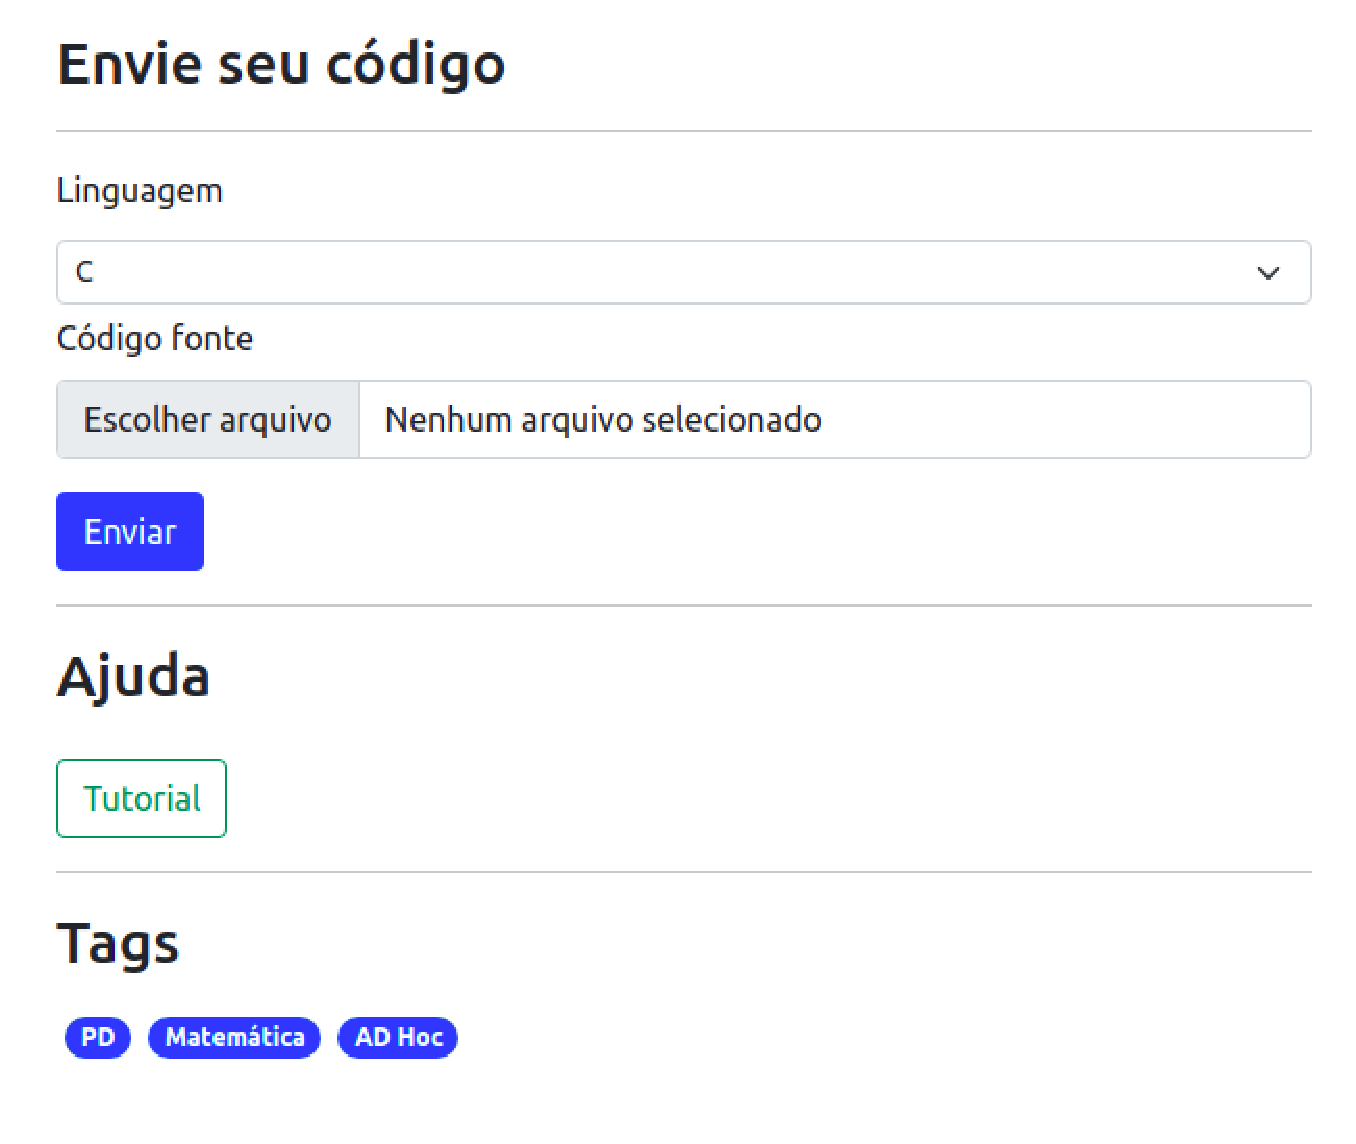
\includegraphics[keepaspectratio=true,scale=0.5]{figuras/sendQuestion1.eps}
    \label{fig:sendQuestion1}
\end{figure}
\begin{center}
    {\tiny Fonte: elaboração nossa}
\end{center}
    
\begin{figure}[H]
    \centering
    \caption{Interface - entradas e saídas da questão}
    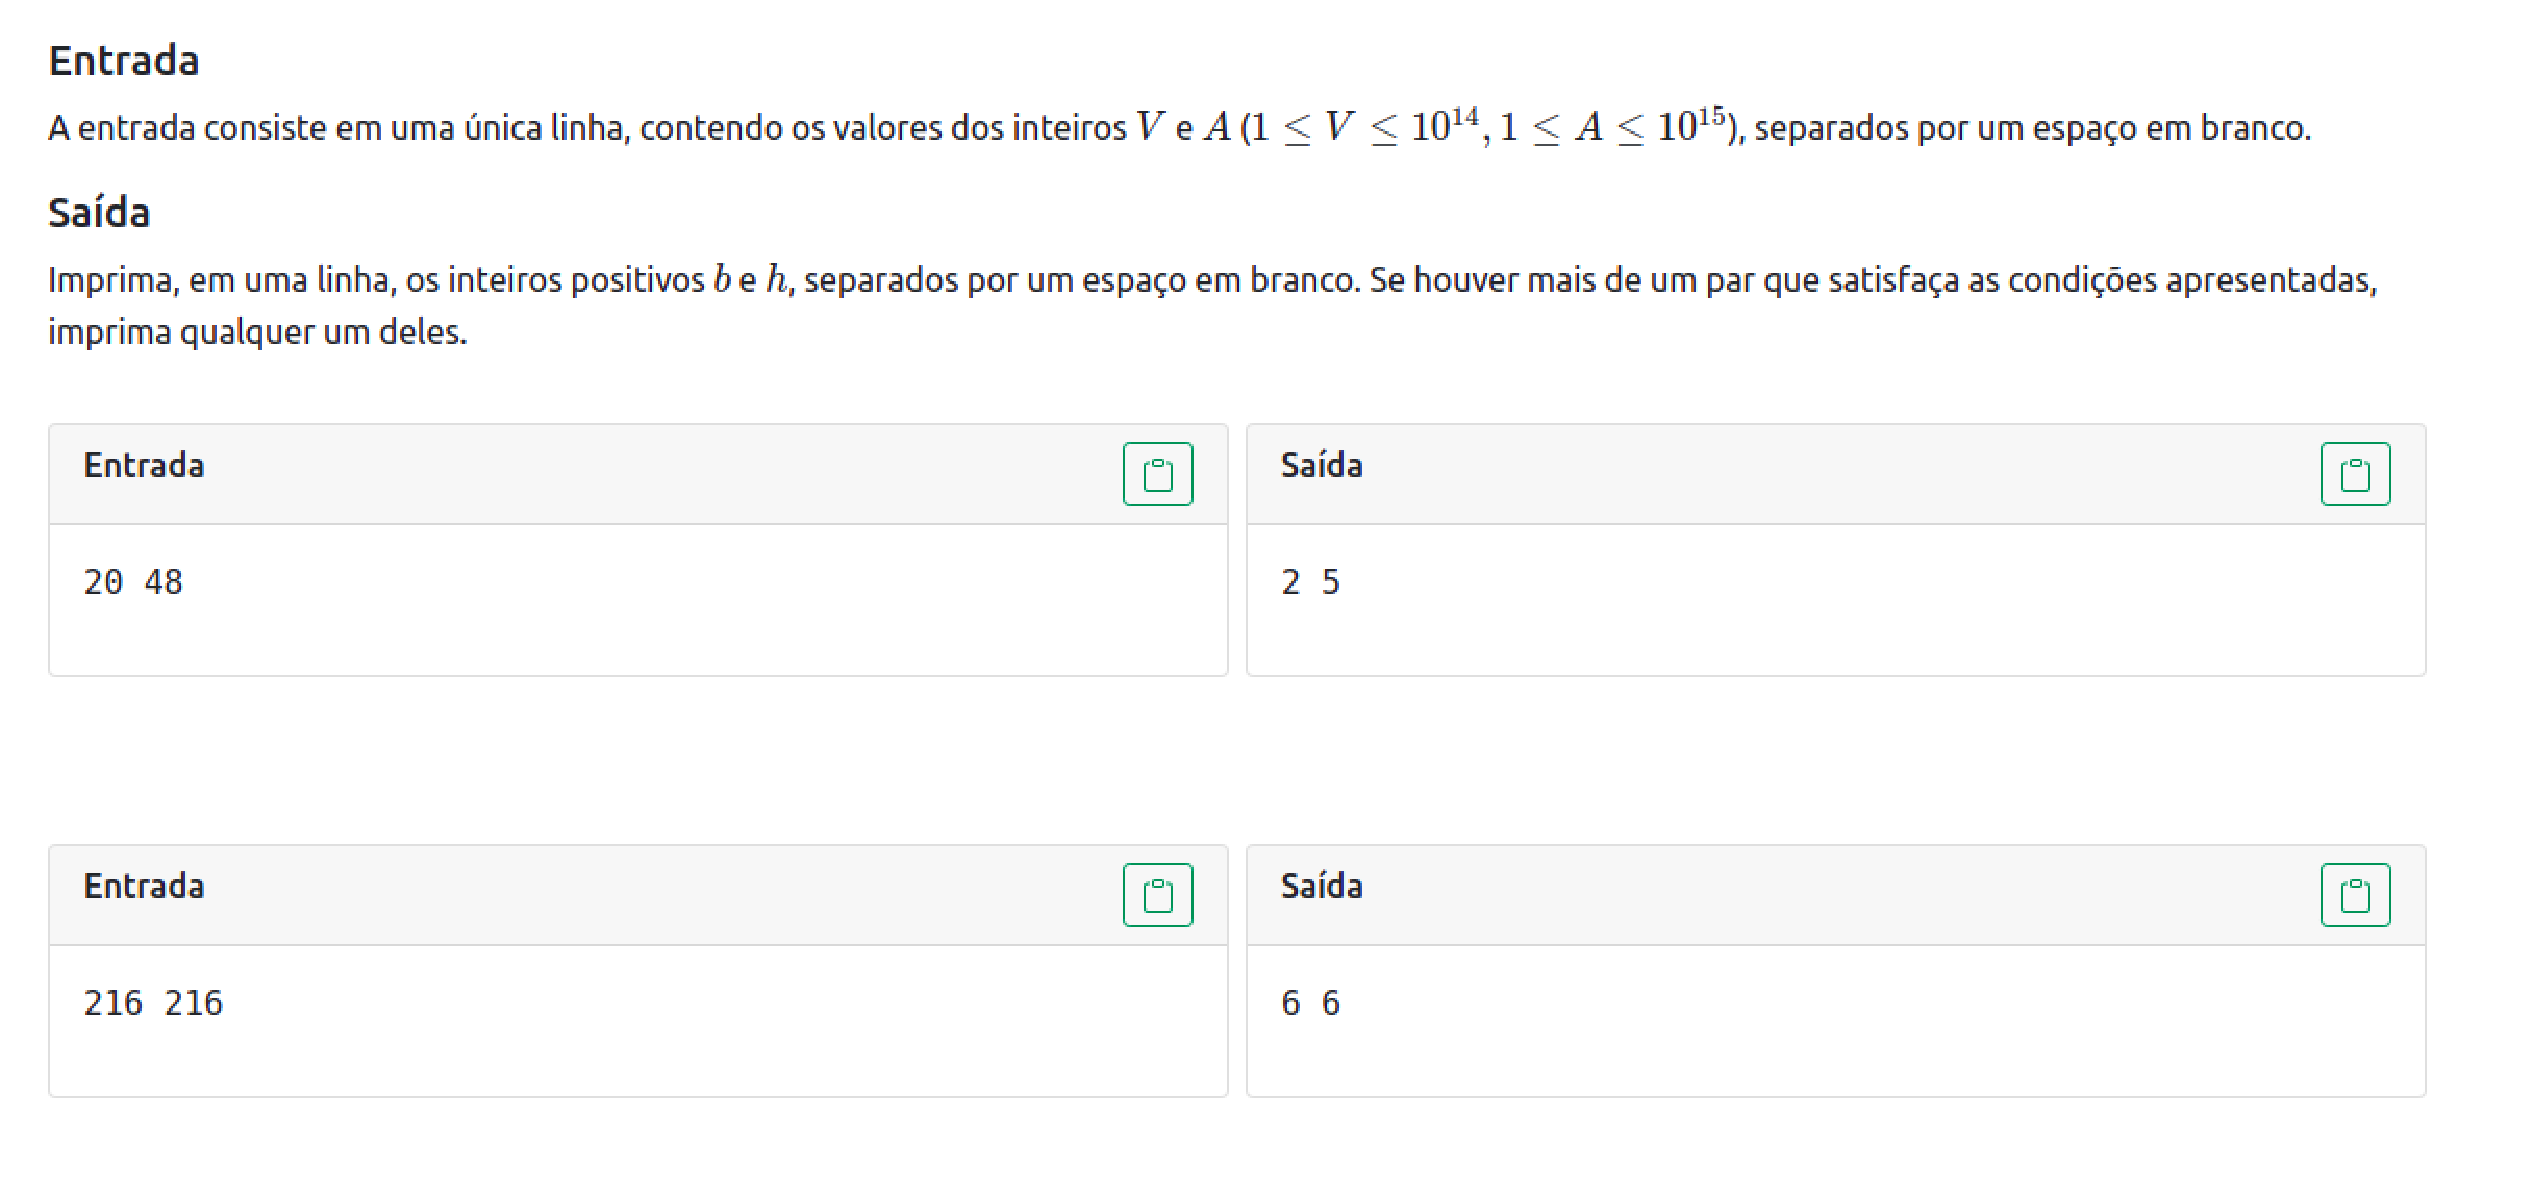
\includegraphics[keepaspectratio=true,scale=0.35]{figuras/questionInputs.eps}
    \label{fig:questionInputs}
\end{figure}
\begin{center}
    {\tiny Fonte: elaboração nossa}
\end{center}

\begin{figure}[H]
    \centering
    \caption{Texto bruto enunciado}
    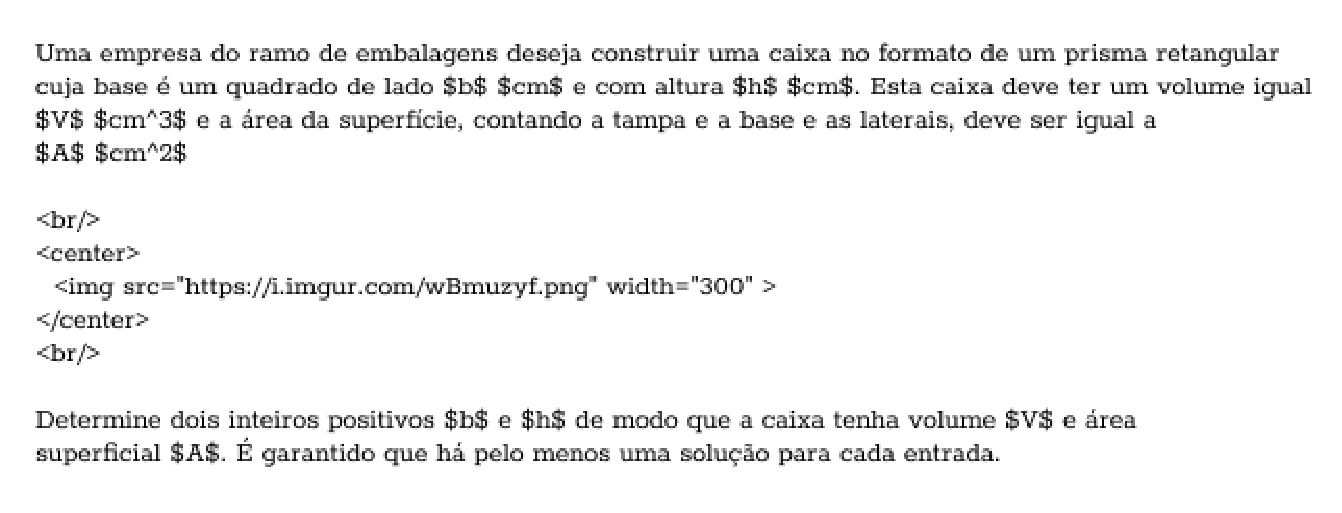
\includegraphics[keepaspectratio=true,scale=0.65]{figuras/statementText.eps}
    \label{fig:statementText}
\end{figure}
\begin{center}
    {\tiny Fonte: elaboração nossa}
\end{center}

\begin{figure}[H]
    \centering
    \caption{Interface - Enunciado da questão}
    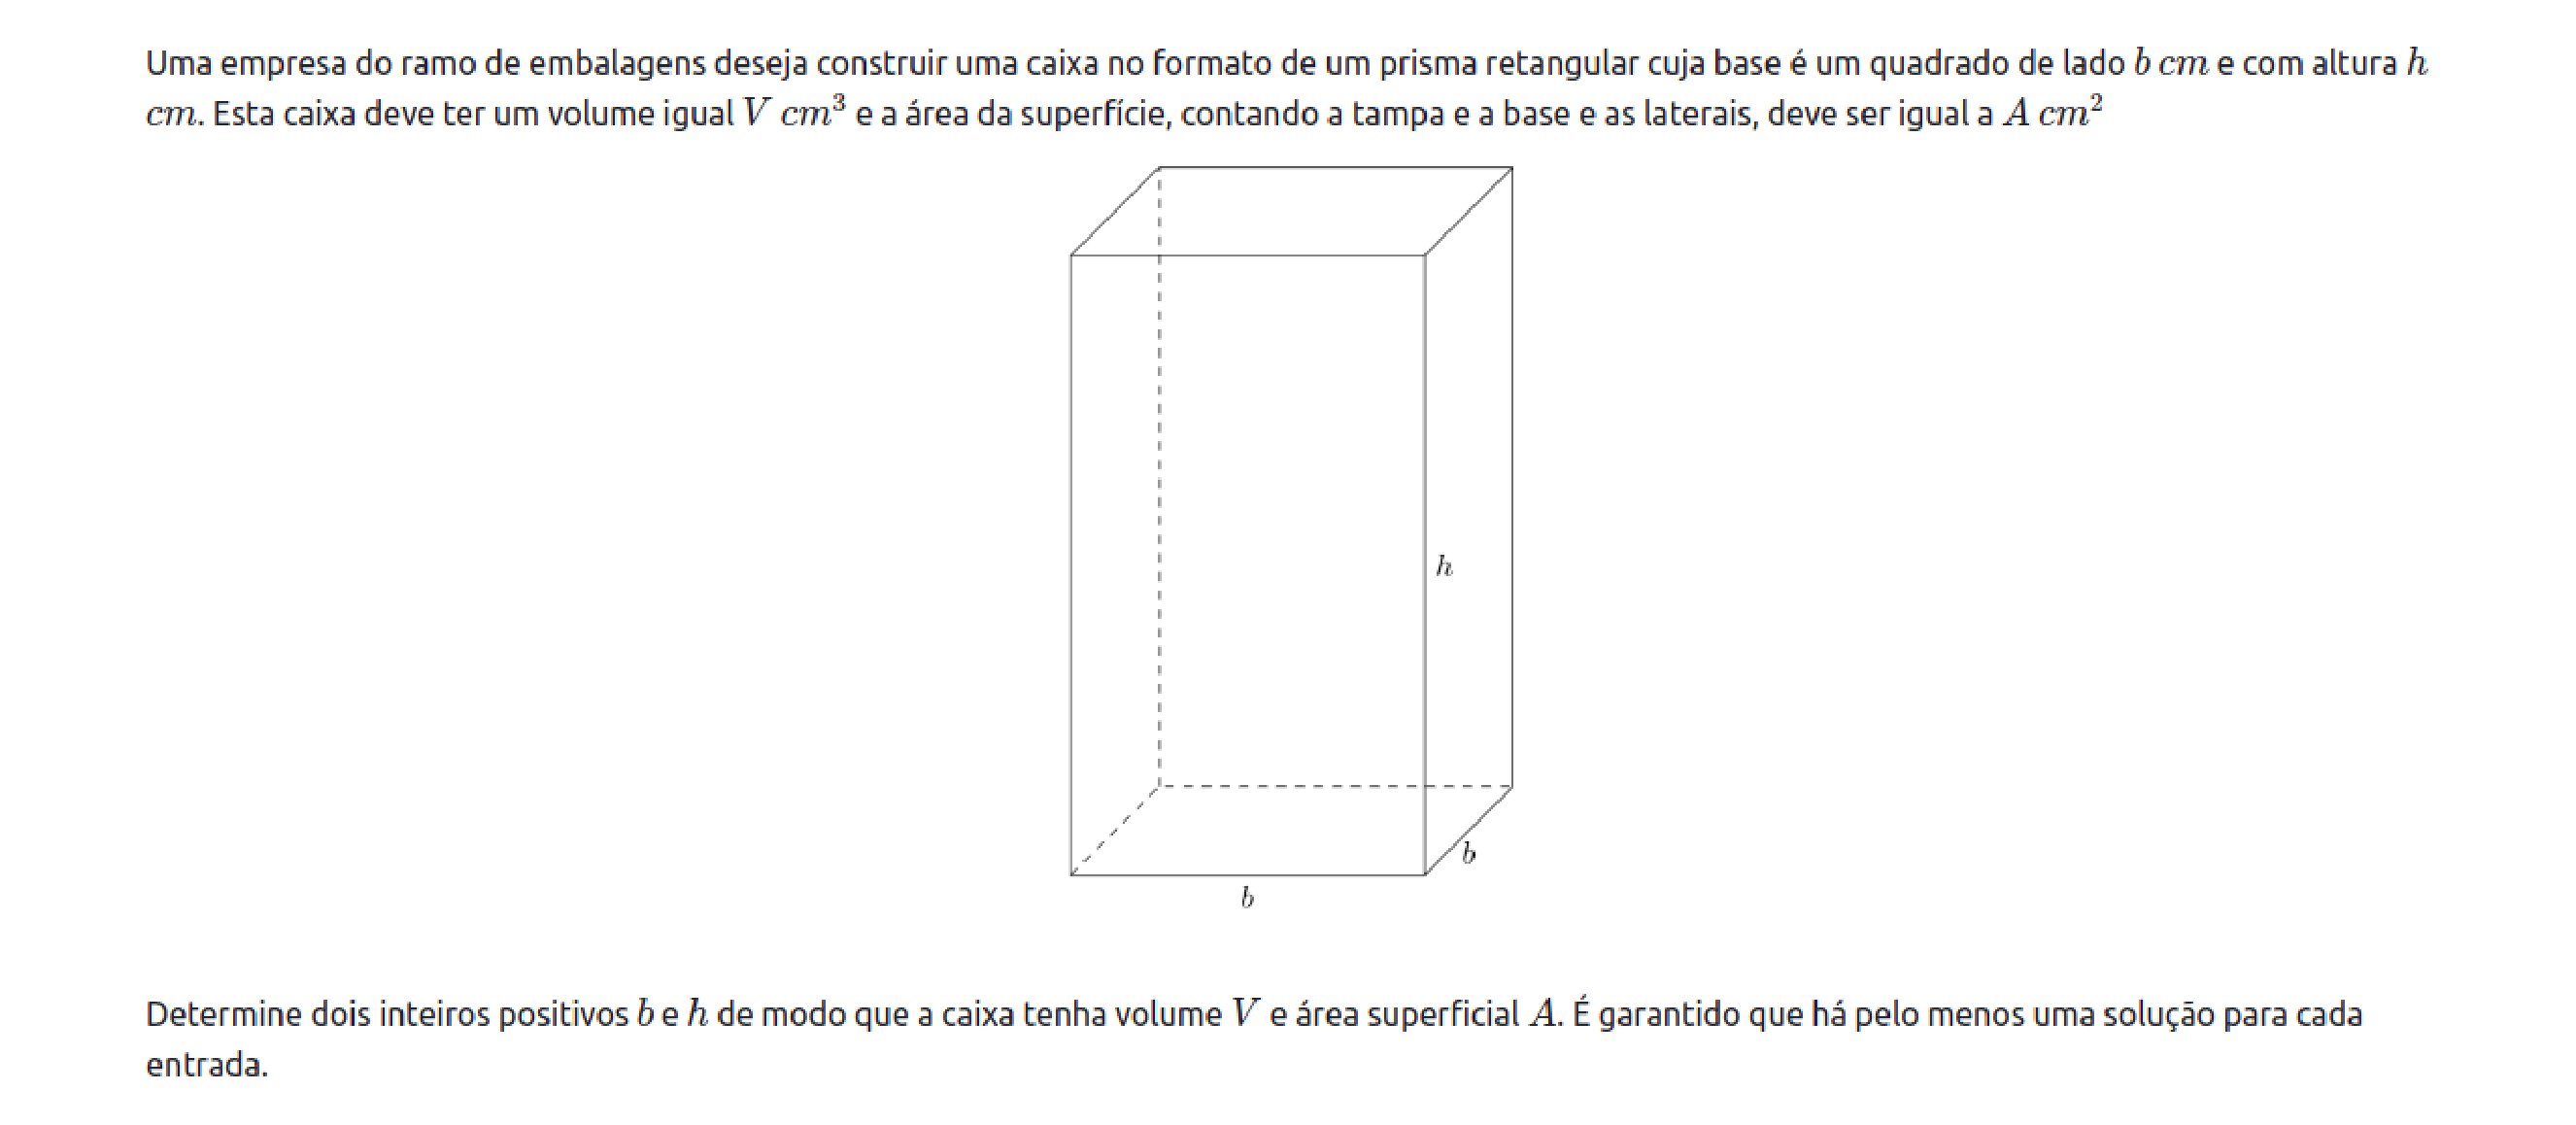
\includegraphics[keepaspectratio=true,scale=0.35]{figuras/questionStatement2.eps}
    \label{fig:questionStatement2}
\end{figure}
\begin{center}
    {\tiny Fonte: elaboração nossa}
\end{center}

\chapter{Scripts}
\label{appendix:b}

\section{Script para coletar número de problemas - Online Judge}
\label{appendix:script_oj}

\begin{lstlisting}[language=Python]

import urllib.request, urllib.error, urllib.parse
from bs4 import BeautifulSoup
import threading

sem = threading.Semaphore()

BASE_URL = 'https://onlinejudge.org/'
MAX_THREADS = 10

def get_soup(url):
    html = urllib.request.urlopen(url).read()
    return BeautifulSoup(html, 'html.parser')

def isProblemCategory(tag):
    try:
        return 'sectiontableentry' in tag['class'][0]
    except:
        return False

def getProblemsCategory(soup):
    return list(filter(lambda tag: isProblemCategory(tag), soup.find_all('tr')))

links_set = set()

def getCategoryLinks(soup):
    link_list = []
    categories = getProblemsCategory(soup)
    for category in categories:
        for tag in category.find_all('a'):
            try:
                link = tag['href']
                if link not in links_set:
                    sem.acquire()
                    link_list.append(link)
                    links_set.add(link)
                    sem.release()
            except:
                pass
    return link_list

links = ['index.php?option=com_onlinejudge&Itemid=8']
threads = []
def processLink(url, links):
    soup = get_soup(url)
    otherLinks = getCategoryLinks(soup)
    sem.acquire()
    links += otherLinks
    sem.release()

while len(links) > 0:
    selected_link = links.pop(0)
    if 'https://www.udebug.com/UVa' in selected_link:
        continue
    if 'page=show_problem' in selected_link:
            print(selected_link)
            continue
    url = BASE_URL + selected_link

    t = threading.Thread(target=processLink, args=(url, links))
    t.start()
    threads.append(t)
    if len(links) == 0 or len(threads) > MAX_THREADS:
        threads.pop(0).join()

for t in threads:
    t.join()
    
\end{lstlisting}

\end{apendicesenv}
